\section{ОБЗОР ЛИТЕРАТУРЫ}
\label{sec:domain}

\subsection{Обзор существующих технологий}
\label{sub:domain:technologies_review}

Современные методы обработки изображений делятся на две основные категории: программная и аппаратная обработка.

Программная обработка производится на базе центрального процессора (CPU) и отличается высокой эффективностью
при использовании последовательных алгоритмов \cite{asano_dip_comp}. В задачах с высоким \en{Data Level Parallelism} по обработке гомогенных данных
центральный процессор значительно проигрывает более специализированным решениям,
из-за малого количества SIMD блоков для параллельной обработки данных \cite{axell_cpu_simd}.

Комбинация программных и аппаратных подходов лежит в основе обработки изображений на графическом процессоре (GPU).
Связка графического процессора и SDK для его программирования образует GPGPU (General-Purpose computing for GPU).
GPGPU основана на принципе SIMT, основанный на разделении задачи на несколько подзадач того же типа, но меньшего размера,
решаемые каждым потоком GPU по отдельности.
Такой подход является удачной комбинацией скорости разработки программы и специализации графического процессора
на параллельной обработке данных \cite{patterson_hennessy}.

Однако есть и существенные ограничения.
Латентность при обработке изображений на GPU слабодетерменирована, что усложняет использование GPGPU
в системах реального времени \cite{maceina_gpu_real_time}.
Отсутствует выбор периферийного интерфейса -- на момент написания,
графический процессоры подключаются исключительно по PCIe (PCI express), сильно ограничивая перечень устройств.
Соотношение производительности на ватт затрудняет применение во встраиваемых системах с автономным питанием \cite{fowers_gpu_power_consumption}.

ASIC (Application-Specific Integrated Circuit), как наиболее специализированное на конкретной задаче решение, выполняет обработку за минимально возможное время
и с минимальным энергопотреблением \cite{amara_asic_low_power}. Разработка специализированной интегральной схемы связана
с существенными затратами на проектирование --- окупаемость наступает лишь при выпуске партиями в несколько сотен тысяч единиц,
исключая возможность применения технологии малыми и средними предприятиями \cite{smith_asic_economy}.

Применение FPGA (Field Programmable Gate Array) достичь баланса между производительностью и конфигурируемостью конечного решения.
По сравнению с ASIC единовременные затраты на проектирование на несколько порядков ниже,
что идеально подходит для прототипирования и мелкосерийного производства \cite{zuchowski_asic_vs_fpga_cost}.
В отличие от GPU малое энергопотребление и небольшие размеры решений на FPGA прекрасно подходят
для встраиваемых систем \cite{berten_gpu_fpga_comparison}.
Последовательные алгоритмы, непригодные для реализации на GPU, могут выполняться
на интегрированном CPU или soft core процессоре, заметно упрощая передачу данных
между последовательным и параллельным вычислителем, решая подобную задачу
для связки GPU и CPU \cite{russo_softcore_fpga_vs_gpu}.

Таким образом, оптимальной технологией для реализации аппаратной системы обработки видеопотока,
с поддержкой модульности и достаточного быстродействия является технология FPGA.


\subsection{Технология FPGA}
\label{sub:domain:fpga}

FPGA (Field Programmable Gate Array) --- программируемые пользователем вентильные матрицы,
представляет собой наиболее общий и современный класс программируемой логики.
Основные области применения FPGA:
\begin{itemize}
  \item разработка блоков и систем на стадии их прототипирования, даже при дальнейшей их реализации на другой технологической базе;
  \item реализация конечных продуктов небольшого тиража, уменьшая затраты на проектирование до возможного минимума.
\end{itemize}

Данные характеристики обеспечиваются удачной комбинацией общих и узкоспециализированных средств
в пределах одной микросхемы. Внутренняя область FPGA содержит множество идентичных конфигурируемых логических блоков (КЛБ),
которые соединены трассами межсоединений. По периметру микросхемы расположены блоки ввода-вывода (БВВ).

Базовая структура FPGA приведена на рисунке~\ref{fig:domain:fpga:fpga_architecture}

\begin{center}
  \centering
  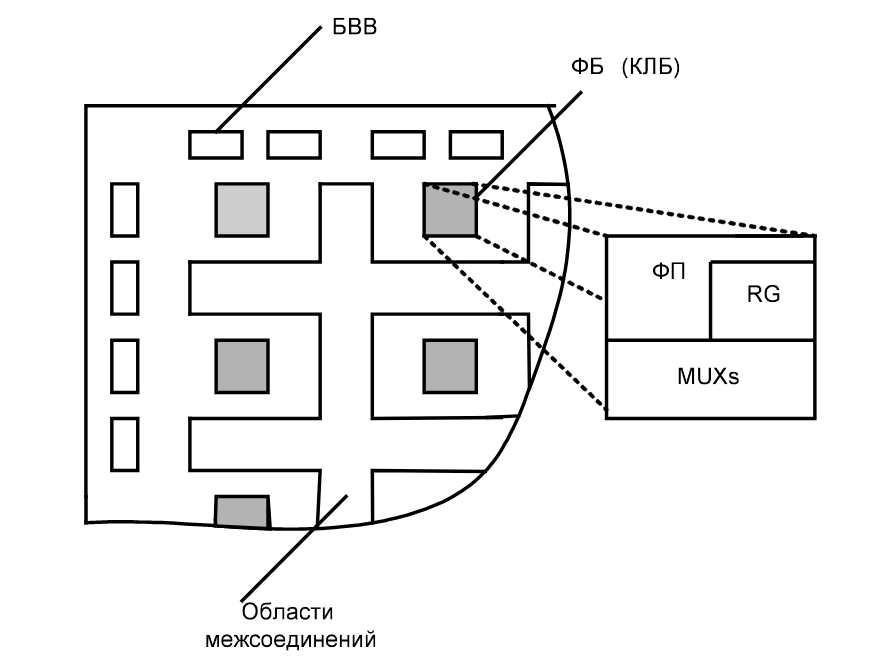
\includegraphics[scale=0.4]{ugrymov_fpga_artchitecture.png}
  \captionof{figure}{ Фрагмент базовой архитектуры FPGA \cite{ugrymov_digital_circuit_engineering} }
  \label{fig:domain:fpga:fpga_architecture}
\end{center}

Конфигурируемые логические блоки состоят из:
\begin{itemize}
  \item некоторого количества элементов выполняющих логические преобразования;
  \item набора мультиплексоров для перенаправления выходных сигналов логических преобразователей;
  \item триггеров для хранения значений сигналов.
\end{itemize}

Схема современного КЛБ на примере семейства Spartan компании \en{Xilinx} представлена на рисунке~\ref{fig:domain:fpga:clb}

\begin{center}
  \centering
  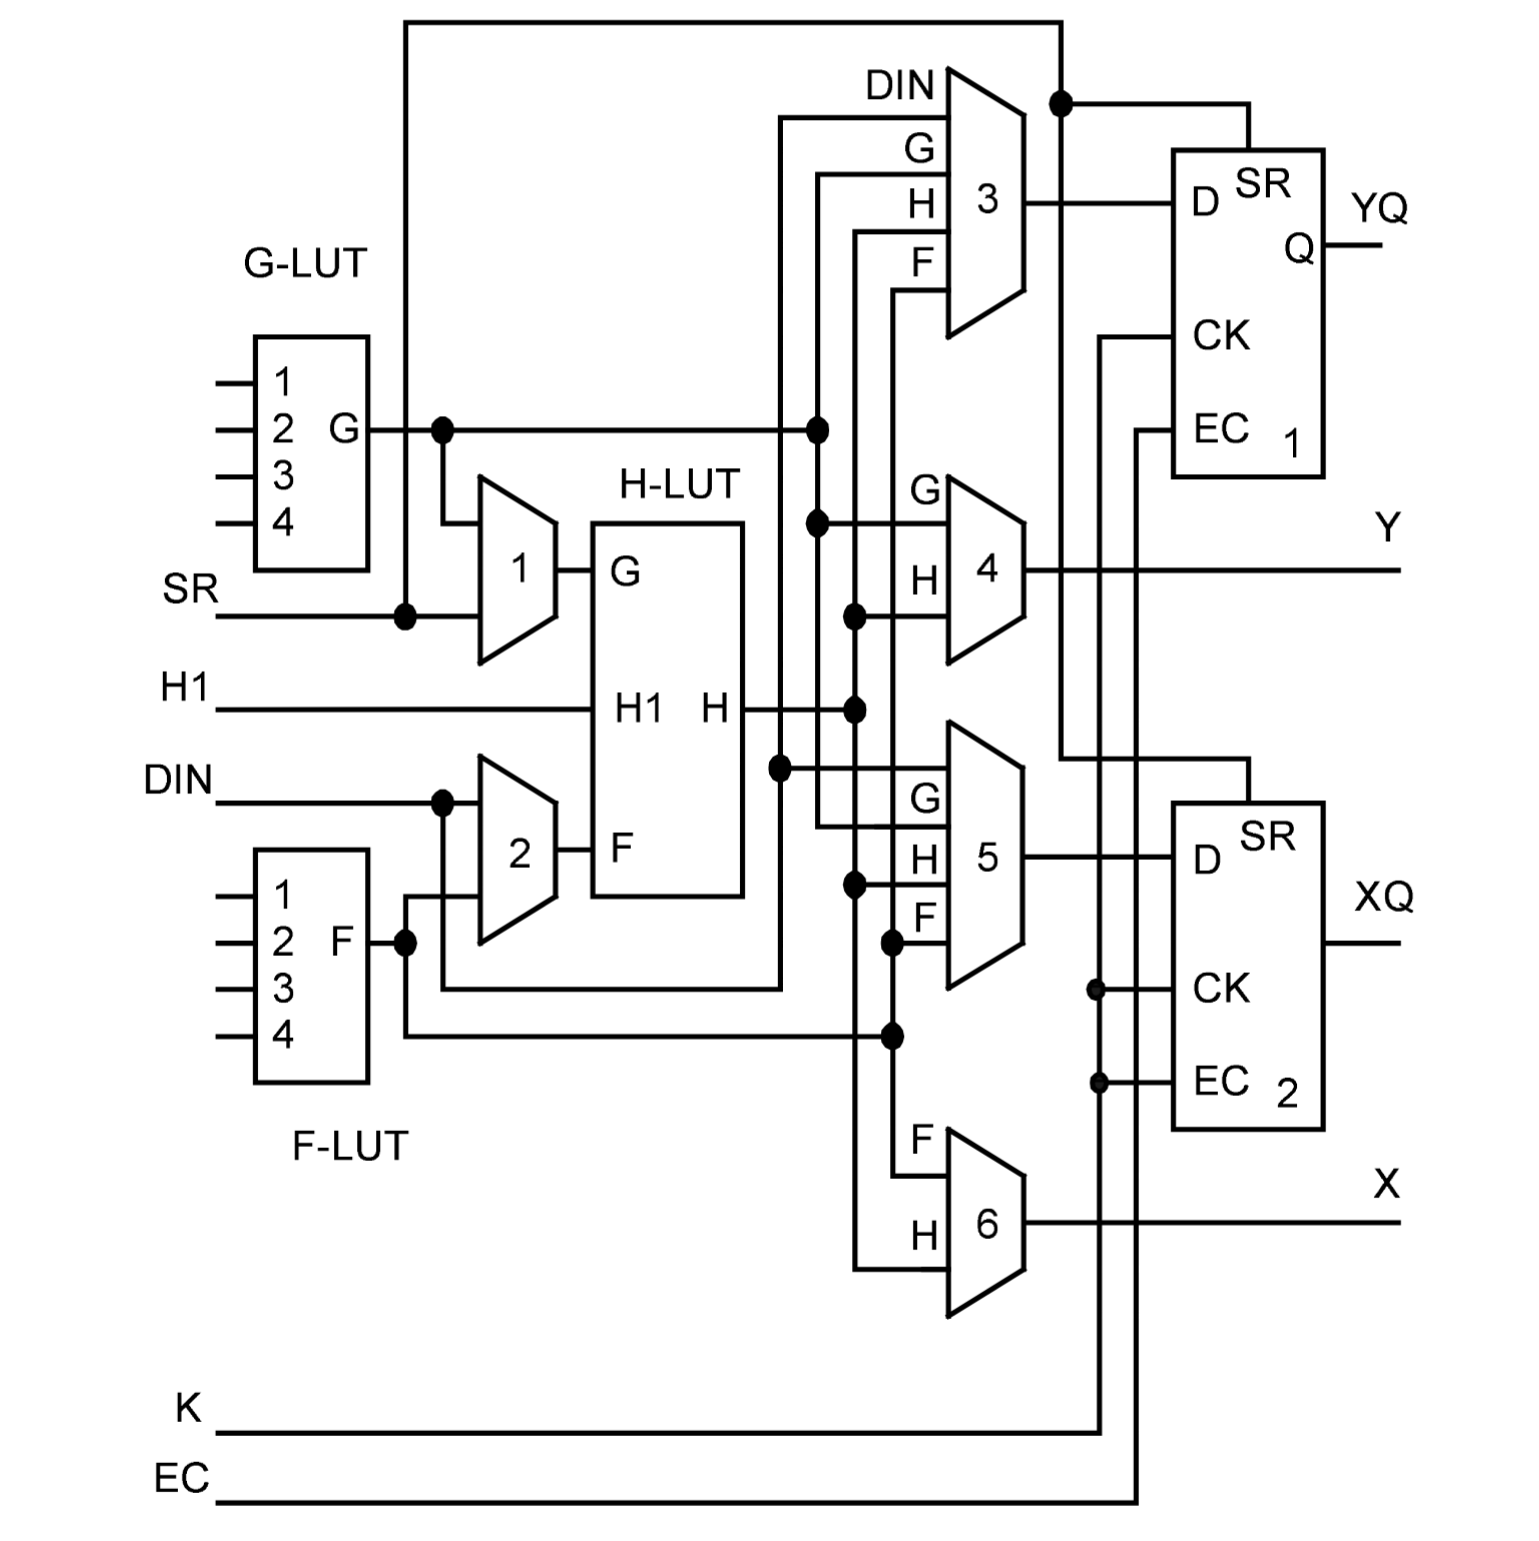
\includegraphics[scale=0.28]{ugrymov_fpga_clb.png}
  \captionof{figure}{ Логический блок семейства Spartan }
  \label{fig:domain:fpga:clb}
\end{center}

Системы межсоединений проектируются в широком диапазоне технологических и архитектурных решений.
Основная цель при построении эффективной системы коммутации --- обеспечение максимальной коммутируемости блоков
при минимальном количестве элементов связи с предсказуемыми задержками сигналов. Обозрение данной тематики задача достаточно нетривиальная,
стоит лишь отметить, что предсказуемость задержек это ключевой фактор в выборе микросхемы для проектирования системы реального времени.

С каждым выводом микросхемы ассоциируется свой блок ввода-вывода, который может настраиваться как вход, выход или двунаправленный вывод.
Упрощенная схема блока В/В представлена на рисунке~\ref{fig:domain:fpga:io}

\begin{center}
  \centering
  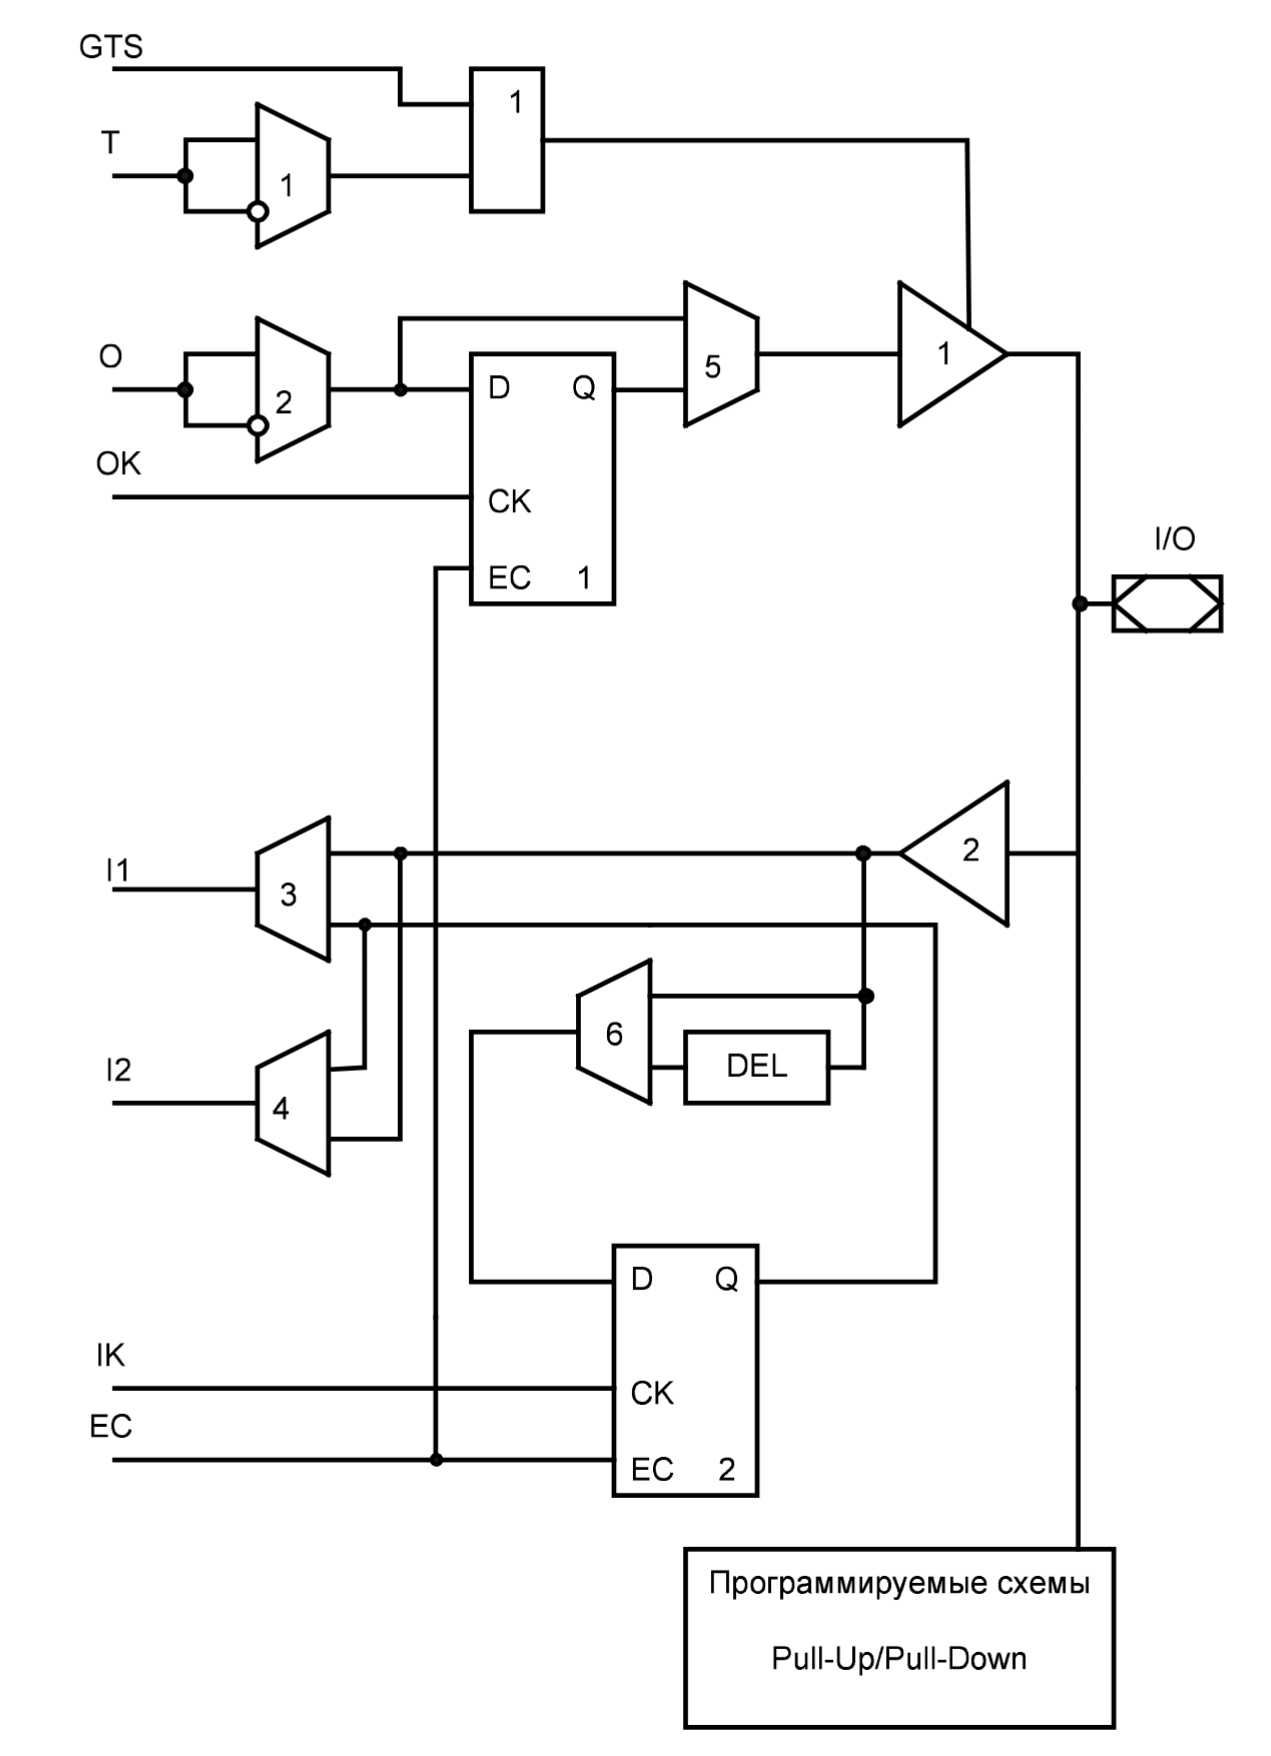
\includegraphics[scale=0.25]{ugrymov_fpga_io.png}
  \captionof{figure}{ Пример схемы блока ввода-вывода FPGA }
  \label{fig:domain:fpga:io}
\end{center}

Блок разделен на две части для работы как на вход, так и на выход. Основной интерес представляют буферы с тремя состояниями
1 и 2. Они имеют программируемые уровни сигналов(КМОП или ТТЛ), что заметно упрощает подключение пользовательских периферийных устройств
напрямую к микросхеме без подключения внешнего преобразователя уровня.

Основными игроками на рынке микросхем FPGA являются Xilinx и Altera. Они производят чипы применимые как в военной и космической сферах,
так и для потребительских нужд. Микросхемы широко варьируются по количеству логических блоков, размеру
статической памяти, количеству блоков ввода-вывода и поддержкой специфических блоков.

Однако для проектирования и отладки системы важен выбор не только микросхемы,
но и отладочной платы с необходимым набором периферии. Подробное сравнение отладочных
плат с микросхемами последнего поколения от различных производителей показывает, что
платы с микросхемами \en{Xilinx} наиболее разнообразны и представлены в более широком ценовом диапазоне,
чем платы Altera \cite{fpga_boards_comparison}.
Вследствие чего сделан выбор применения микросхем Xilinx в дипломном проекте.

\subsection{Сравнение cемейств микросхем Xilinx}
\label{sub:domain:fpga_comparison}

Компания Xilix является технологическим лидером на рынке производства микросхем FPGA.
На данный момент наиболее актуальная линейка микросхем --- Xilinx 7 series\cite{7_series_overview}.
Продукты данной линейки покрывают всевозможные требования к микросхеме: от низкого энергопотребления, малого размера, низкой цены до
поддержки высокоскоростных интерфейсов и большого количества логических и DSP (Digital Signal Processing) блоков.

Седьмое поколение микросхем Xilinx делится на 4 основные категории:
\begin{itemize}
  \item Spartan-7: для недорогих и маломощных систем, требующих высокую производительность ввода-вывода.
    Имеет наименьшую площадь посадочного места во всей линейке;
  \item Artix-7: оптимизирован для маломощных приложений с требованиями по высокой пропускной способности логических и DSP блоков.
    Обладает наиболее высоким параметром производительности на ватт;
  \item Kintex-7: микросхема с лучшим соотношением цены к производительности;
  \item Virtex-7: лучшая в классе производительность с применением новейших производственных технологий.
\end{itemize}

Так как в системах обработки видео с помощью FPGA блоки DSP выполняют роль сопроцессора, то
основная нагрузка ложится на саму микросхему. Исходя из этого следует подбирать микросхему
руководствуясь её предельной тактовой частоты и количества логических блоков\cite{7_series_selection_guide}.

Старшие микросхемы в линейке Spartan работают на частотах порядка 500 МГц, однако обладают слишком малым количеством
логических и DSP блоков.

FPGA линейки Virtex являются самым передовым решением компании, их характеристики превосходят необходимые требования,
но стоимость на порядок выше младших решений делает их выбор не оптимальным.

Семейства Kintex и Artix используют 28 нм техпроцесс, основное различие различается в количестве DSP блоков, что не является
ключевым фактором в выборе микросхемы. При схожих параметрах, микросхемы Artix стоят меньше чем Kintex\cite{artix_kintex_price_comparison},
что послужило основанием для выбора данного семейства в дипломном проекте.

% Плюсы fpga конкретно для DIP dark fantasies

% Параллелизм в алгоритмах обработки изображений существует в двух основых формах --- пространственный и временный.
% Реализации данных алгоритмов на FPGA потенциально могут использовать комбинацию двух форм.\cite{downton_dip_architectures}.

% В частости, в задачах обработки изображения, FPGA ценится за возможность применения в системах
% с динамической реконфигрурацией, в которых требуется быстрая смена настроек системы для подстраивания
% под изменяющиеся внешние параметры \cite{burns_fpga_run_time_reconf}.

% Можно добавить отдельную секцию про выбор платы, но это уже занадто

\subsection{Обзор платы AC701}
\label{sub:domain:ac701}

Плата AC701 от компании Xilinx представляет собой так называемый \en{evaluation board},
содержащую все возможные периферийные устройства подключаемые к микропроцессору.
Среди них особый интерес представляют:
\begin{itemize}
  \item микросхема XC7A200T-2FBG676C семейства Artix-7;
  \item 1GB DDR3 SODIMM;
  \item программируемый осциллятор;
  \item FMC (FPGA Mezzanine Card);
  \item шина I2C разведённая ко всей программируемой на плате периферии;
  \item контроллер и коннектор HDMI.
\end{itemize}

Структурная схема платы представлена на рисунке~\ref{fig:domain:ac701:block_design}

\begin{center}
  \centering
  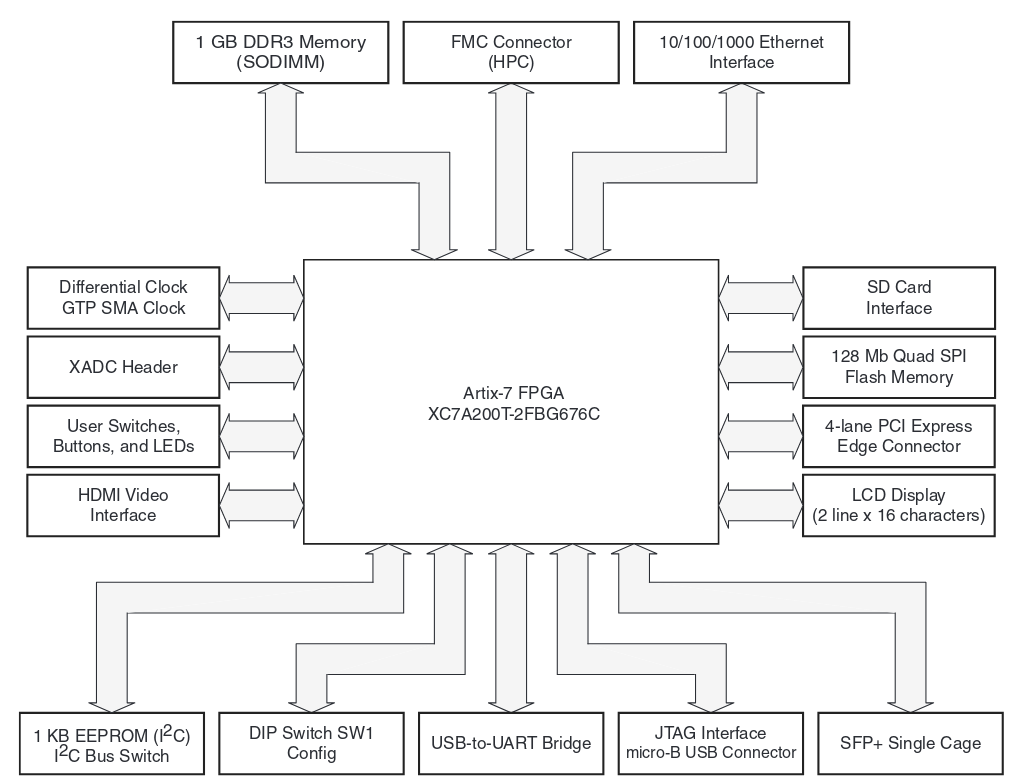
\includegraphics[scale=0.4]{ac701_block_design.png}
  \captionof{figure}{ Блок схема платы AC701 }
  \label{fig:domain:ac701:block_design}
\end{center}

Кадр HDTV видеопотока занимает порядка 1280 $\cdot$ 720 $\cdot$ 3 $=$ 2,76 МБ памяти. Размер SRAM памяти
микросхемы составляет 2,8 МБ, что позволяет буферизировать один кадр видеопотока. Однако большинство
алгоритмов обработки изображений работают со буфером памяти, в котором сохраняются промежуточные результаты
вычислений. Для таких целей объёма SRAM памяти становится недостаточно. Поэтому
для временного хранения потока приходящих кадров необходима динамическая память.   % Можно добавить ссылку на расчёты во введении или привести новые для 2160/1080

Программируемый осциллятор позволяет подключать к дополнительной периферии, например камере, тактовый сигнал произвольной частоты.
Для задания опорной частоты используется шина I2C. Частота варьируется от 10 МГц до 810 МГц. Высокие частоты достигаются применением дифференциальной пары.
Схема осциллятора представлена на рисунке~\ref{fig:domain:ac701:user_clock}

\begin{center}
  \centering
  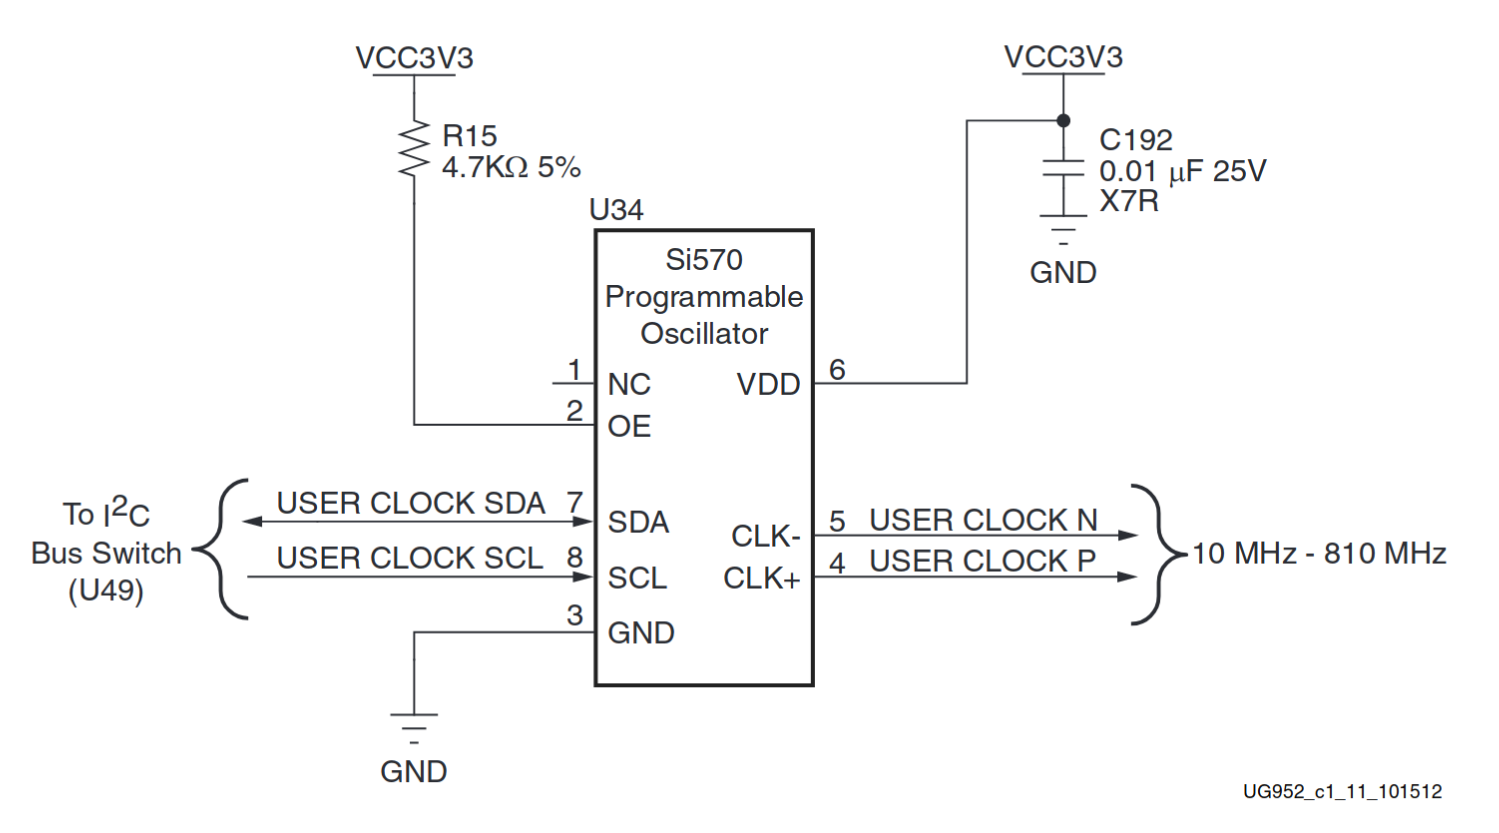
\includegraphics[scale=0.25]{ac701_user_clock.png}
  \captionof{figure}{ Программируемый осциллятор }
  \label{fig:domain:ac701:user_clock}
\end{center}

Подключение произвольных периферийных устройств осуществляется через разъём FMC, поддерживающий передачу
высокочастотных дифференциальный и однополярных сигналов на частотах до 9 ГГц\cite[c. 57]{ac701_user_guide}.
К таким устройствам относятся любые источники высокочастотных данных, такие как камеры, приёмники сигналов и так далее.

Программирование устройств на плате осуществляется посредством записи внутренних регистов по шине I2C. Она служит основным
инструментом настройки и диагностирования состояния компонентов на плате. Точный список устройств показан на
рисунке~\ref{fig:domain:ac701:i2c}

\begin{center}
  \centering
  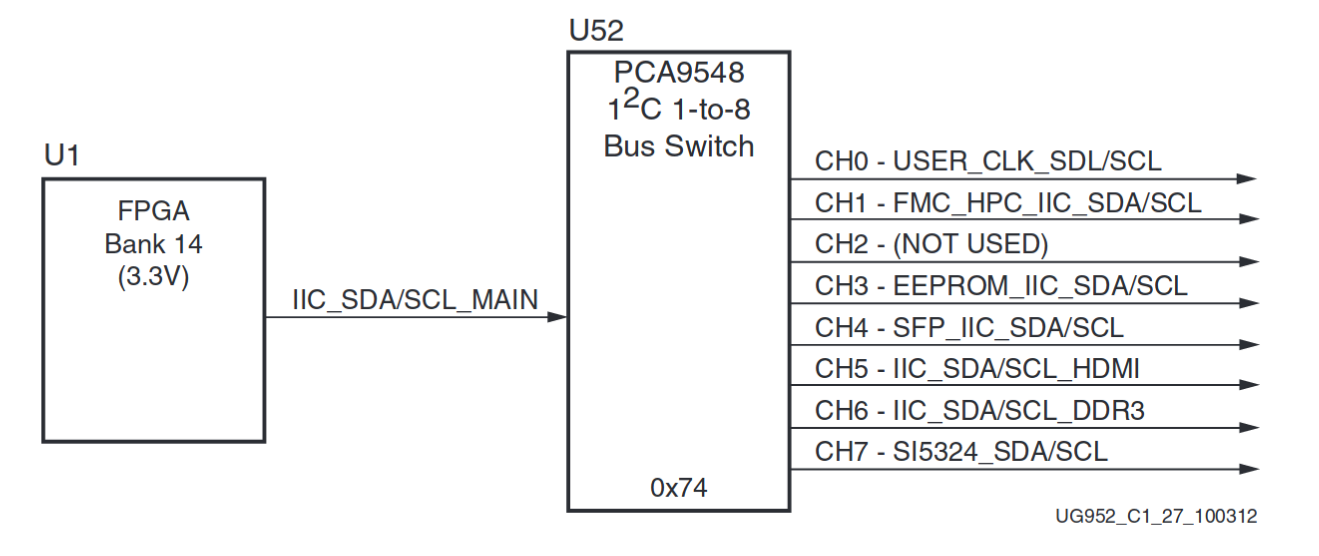
\includegraphics[scale=0.25]{ac701_i2c.png}
  \captionof{figure}{ Топология шины I2C }
  \label{fig:domain:ac701:i2c}
\end{center}

Обработанное видео передаётся через коннектор HDMI (\en{High Definition Multimedia Interface}) на устройство видеовывода либо дальнейшей обработки. В качестве
HDMI контроллера на плате установлен ADV7511KSTZ-P компании Analog Devices. Контроллер поддерживает передачу видео формата 1080p 60 Гц в
цветовом пространстве YCbCr 4:4:4, блоками по 24 бита.
Схема подключения контроллера представлена на рисунке~\ref{fig:domain:ac701:hdmi}

\begin{center}
  \centering
  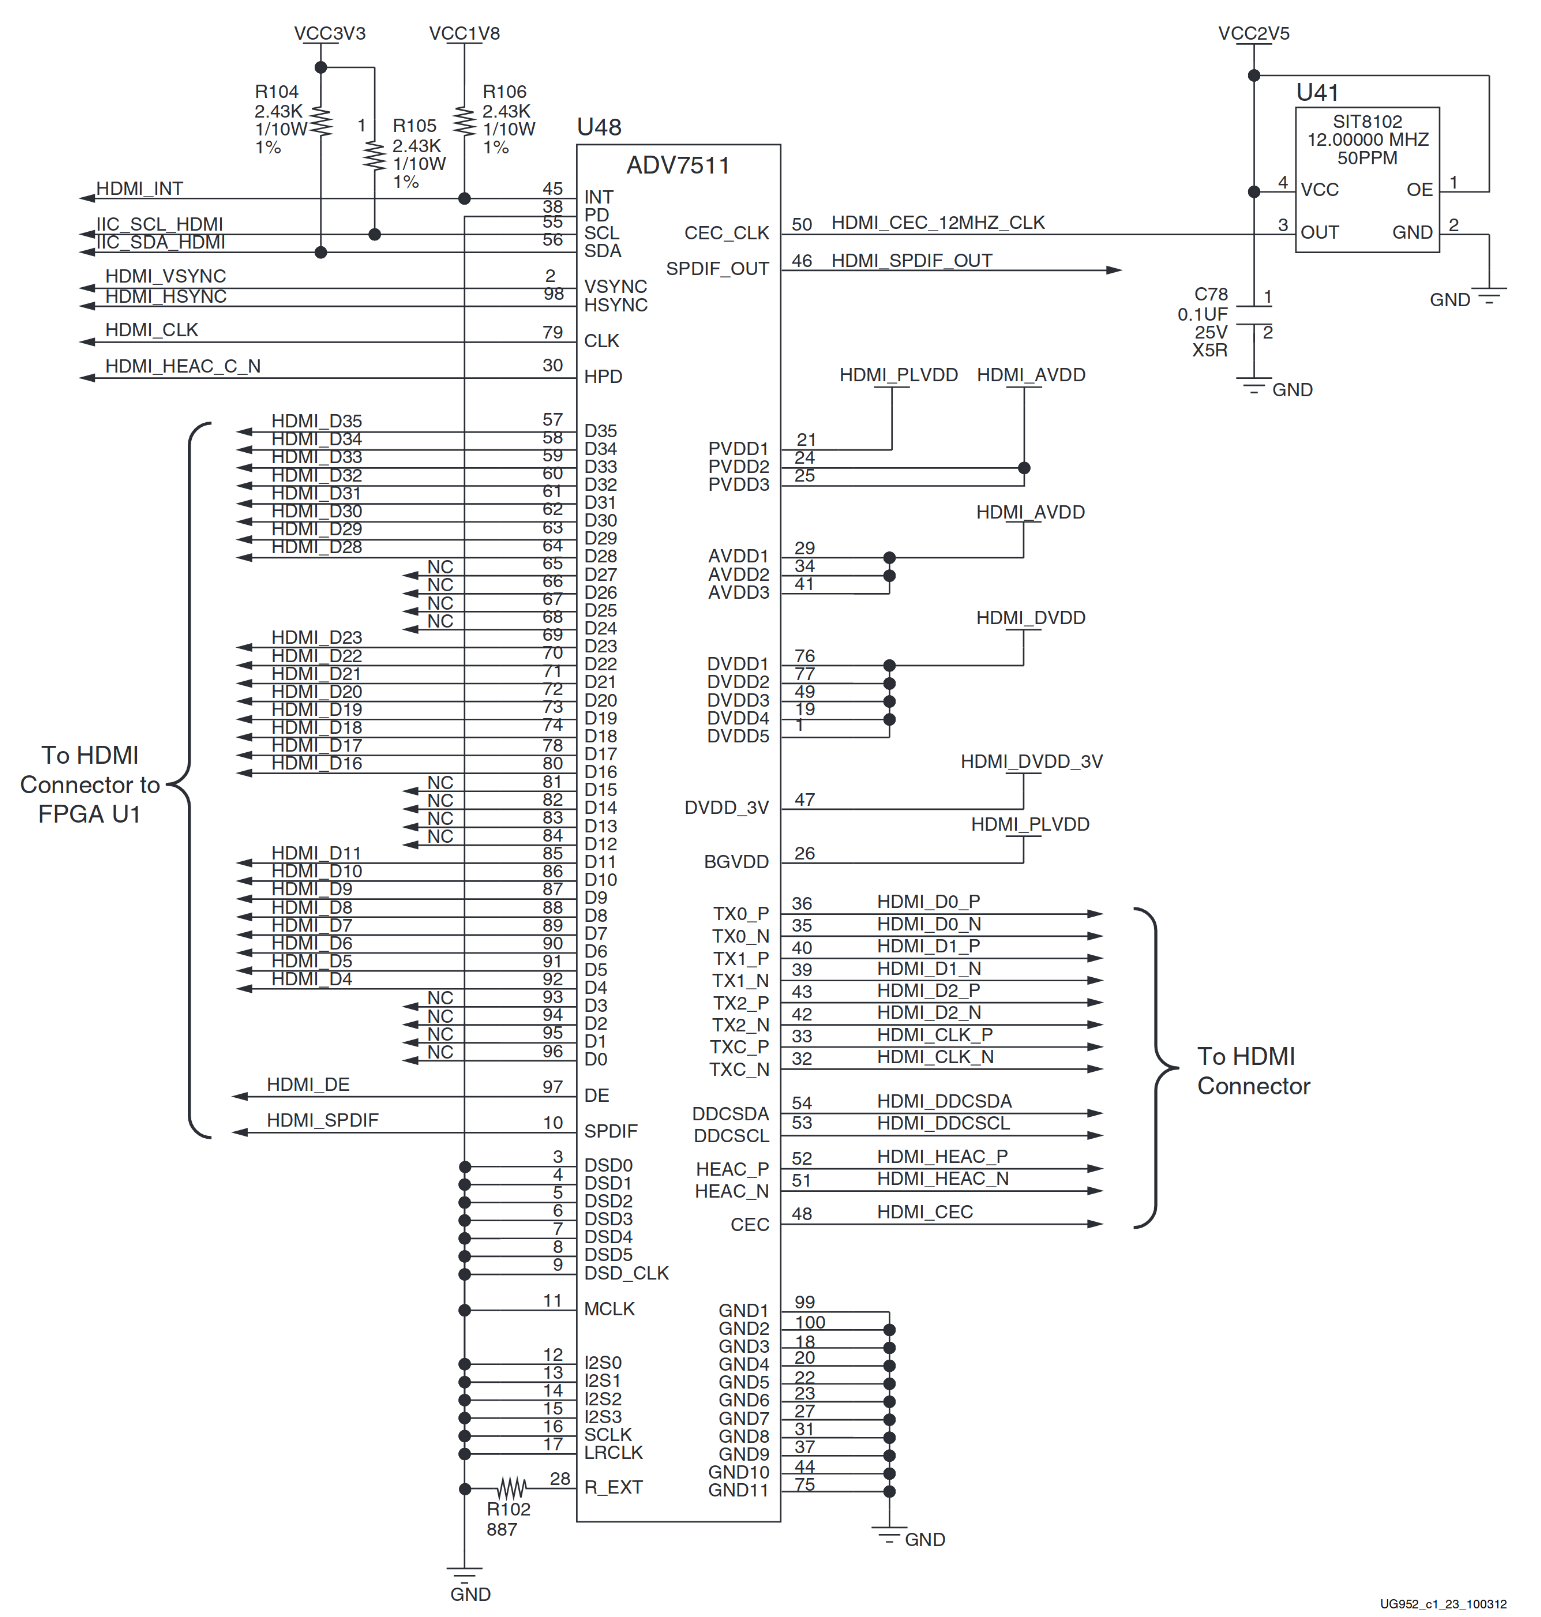
\includegraphics[scale=0.28]{ac701_hdmi.png}
  \captionof{figure}{ Схема подключения HDMI контроллера }
  \label{fig:domain:ac701:hdmi}
\end{center}

Более подробная информация о подключении, назначении внутренних регистров и режимах работы содержится в \cite{adv7511_datasheet}.

\subsection{Обзор камер}
\label{sub:domain:camera}

Одним из источников видео являются видеокамеры.

Оптические сенсоры современных камер производятся по двум технологиям: ПЗС и КМОП.
Основной принцип работы матрицы на приборе с зарядовой связью заключается в сдвиге заряда,
накопленного элементами ПЗС матрицы.
В свою очередь в КМОП-матрицах фоточувствительные элементы являются независимыми друг от друга единицами
и не влияют напрямую на накопленный друг другом заряд.
Несмотря на низкую светочувствительность КМОП-матриц по сравнению с ПЗС, их цена, энергопотребление и
быстродействие почти полностью вытеснили ПЗС-матрицы с рынка потребительской электроники, поэтому
в дальнейшем будут обозреваться КМОП-камеры.

Критерием выбора служит поддержка съёмки видео высокого разрешения (1280x720 HDTV и выше).
Большинство камер поддерживают либо меньшее разрешение, либо поставляются на платах с большим
количеством лишней периферии. Среди подходящих под требование наиболее выделяется модуль
MT9T031C12STCH ES компании Aptina. При разрешении 1280x720 частота кадров достигает 38 снимков в секунду,
что приемлемо для восприятия человеком. Так как современные FPGA работают от напряжения 3.3 В, данная камера
может питаться напрямую от источника питания для платы без преобразований\cite{image_sensor_datasheet}.
Схема подключения камеры представлена на рисунке~\ref{fig:domain:camera:camera_configuration}

\begin{center}
  \centering
  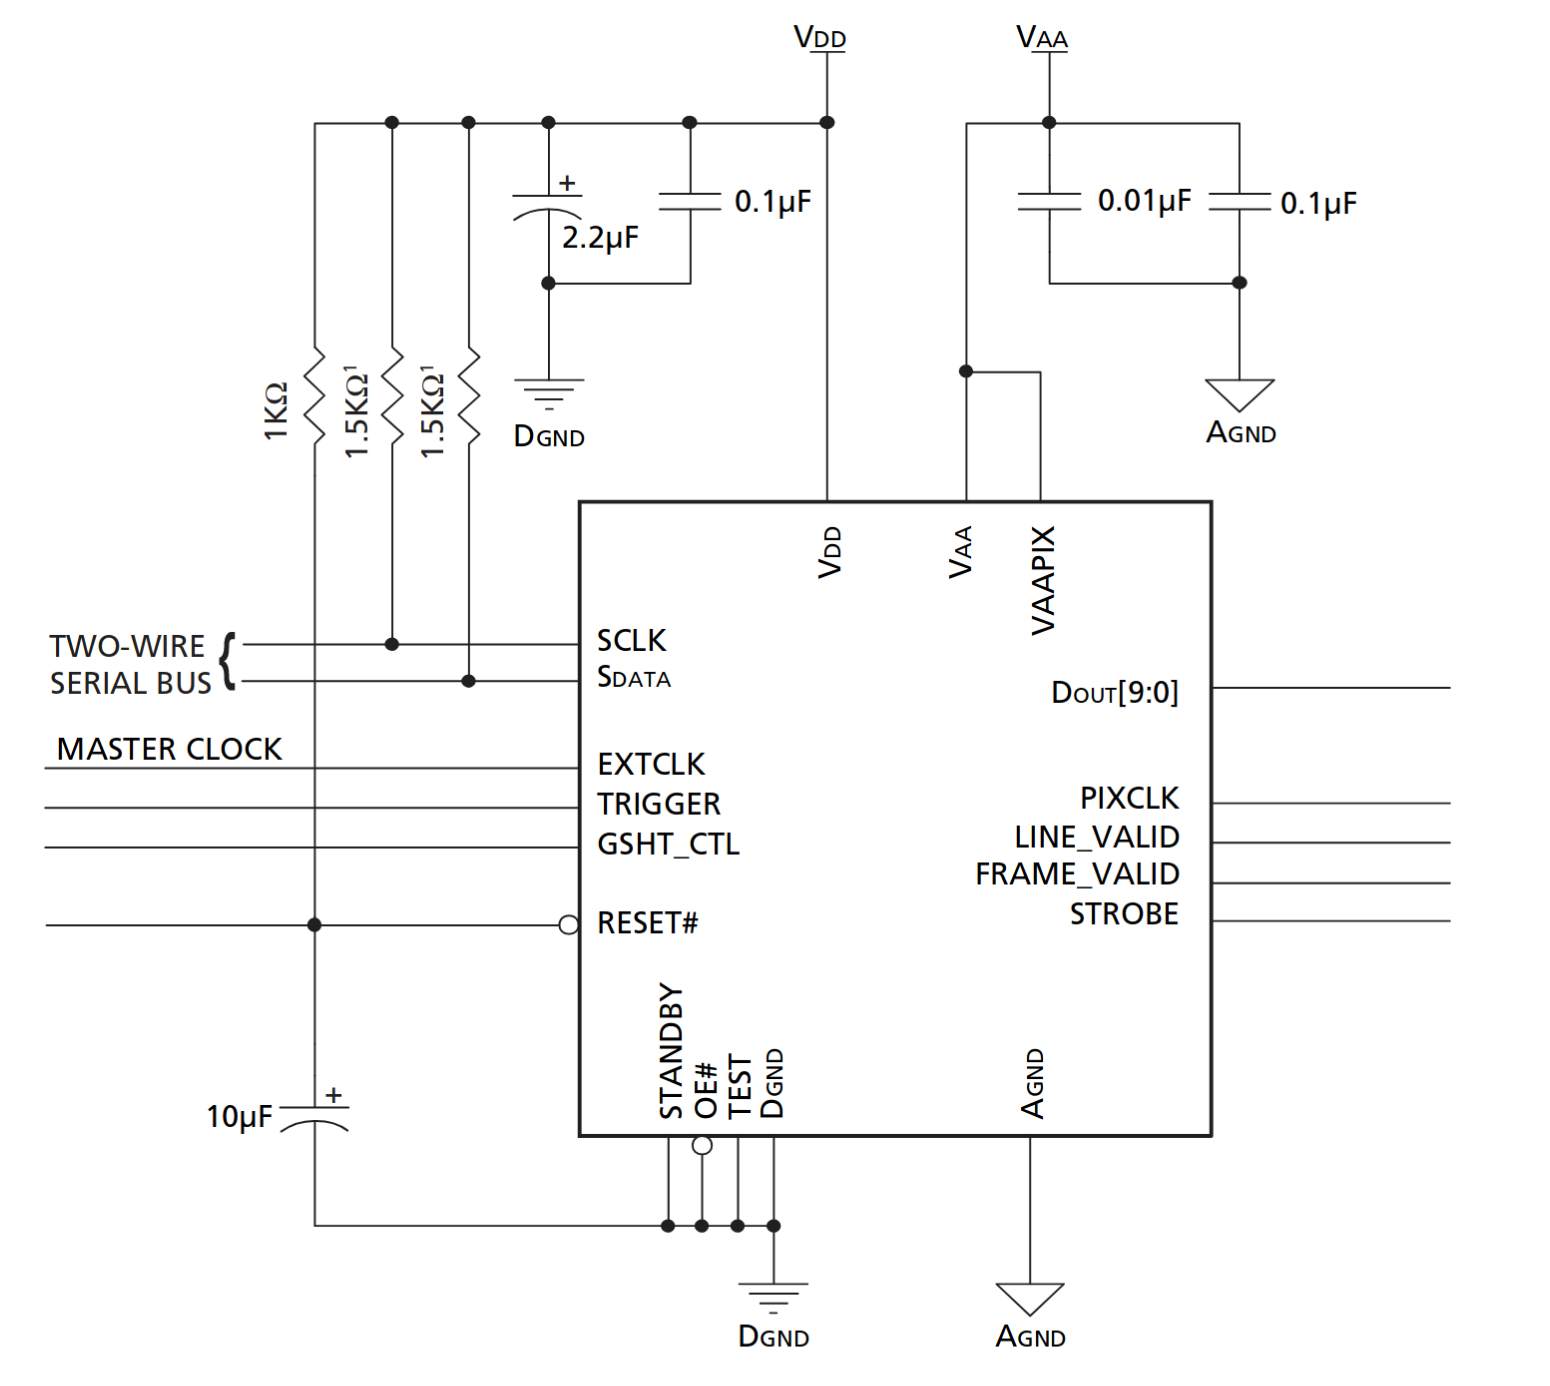
\includegraphics[scale=0.22]{camera_configuration.png}
  \captionof{figure}{ Схема подключения камеры \cite{camera_module_datasheet} }
  \label{fig:domain:camera:camera_configuration}
\end{center}

% Это чтобы не ехали подписи
В качестве синхросигналов используется HSYNC и VSYNC, видеоданные передаются по 10-битной параллельной шине.
Модуль поддерживает различные режимы работы, одним из которых является режим пропуска областей кадра, для
уменьшения объёма передаваемых данных. Настройка камеры производится записью внутренних регистров по протоколу I2C.
% \subsection{Microblaze}
% \label{sub:domain:microblaze}

\subsection{Обзор аналогов}
\label{sub:domain:alternatives}

Системы обработки видео на FPGA получили распространение в конце 1990-ых годов, когда
производство программируемой логики стало коммерчески выгодным. Работы делятся на несколько
направлений: портирование алгоритмов ЦОС с последующими замерами времени выполнения,
проектирование систем реального времени, создание систем обработки видео для встраиваемых систем.

Данные системы, как правило, не обладают модульной архитектурой: попытка внесения изменений,
например, добавление нового фильтра в цепочку обработки, требует изменения большей части
составных блоков.
К примеру, в работе \cite{meng_fpga_based_video_processing} разработанная система
имеет линейную архитектуру, не предполагая наличия управляющей логики, что существенно сужает круг
её применения. Архитектура линейной системы представлена на рисунке~\ref{fig:domain:alternatives:linear_architecture}

\begin{center}
  \centering
  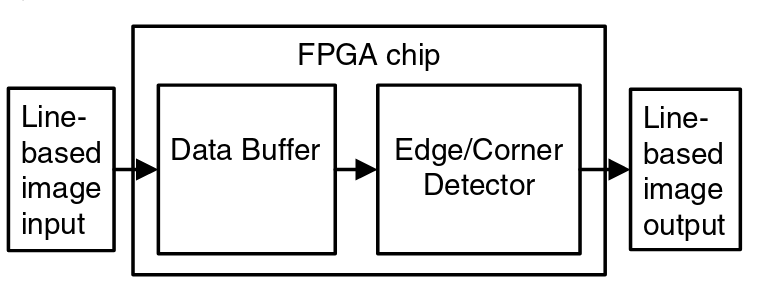
\includegraphics[scale=0.28]{system_linear_architecture.png}
  \captionof{figure}{ Архитектура линейной системы обработки видео }
  \label{fig:domain:alternatives:linear_architecture}
\end{center}

Другие системы \cite{embeded_real_time_fpga_modular} разделяют управляющую
и обрабатывающую логику, однако не поддерживают добавления блоков обработки в произвольное
место в потоке данных(перед конвертацией видео во внутренний формат FPGA или после).
Схема данной системы представлена на рисунке~\ref{fig:domain:alternatives:microblaze_architecture}

\begin{center}
  \centering
  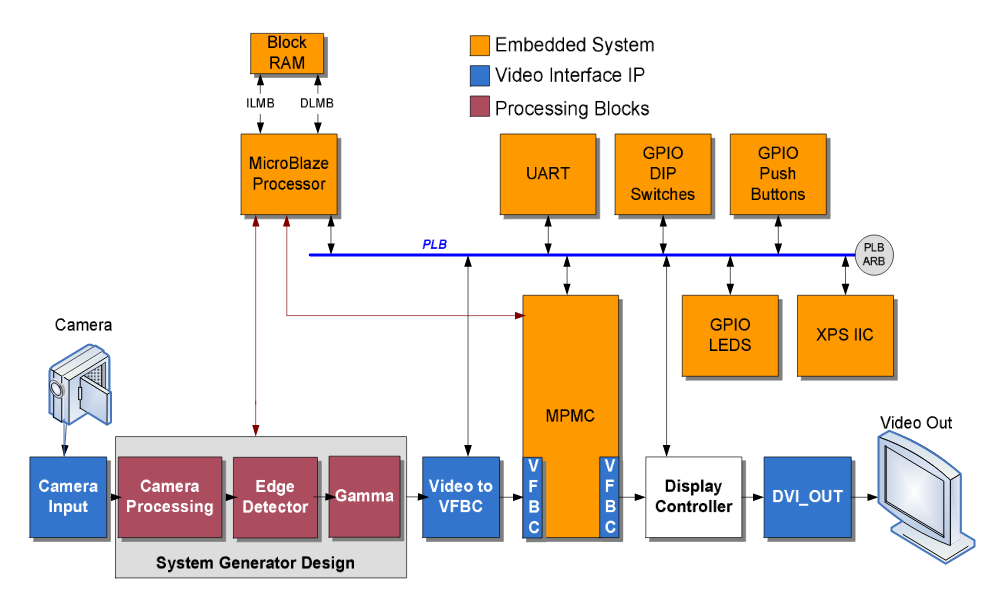
\includegraphics[scale=0.3]{system_microblaze_architecture.png}
  \captionof{figure}{ Потоковая система обработки видео }
  \label{fig:domain:alternatives:microblaze_architecture}
\end{center}

Наиболее удачным решением является комбинация линейной системы, поддерживающей интеграцию сторонних модулей в цепь обработки, и
выделенного модуля управления, для настройки и отслеживания состояния системы.
